\chapter{Architecture Description}

This chapter provides a summary of the research done for this thesis as an resulting artefact. This artefact takes the form of an architecture description in accordance to ISO42010 and is expressed in terms of the 4+1 view model. The architecture description is also created through following an attribute-driven design approach. Utimately this chapter aims to provide enough specifics, diagrams and details to be useful in future implementations of a multi-tenant system or prototype. 

\section{Adapted Attribute-Driven Design Approach}
In creating an architecture description, the architect is faced with a range of diverse approaches. Each one of these approaches offers a certain framework for creating the AD and sets certain context and constraints on the design used. One such comprehensive approach to AD design is Attribute-Driven Design (ADD). In its essence, ADD is an approach to defining an AD that uses the software's quality attribute requirements as baseline for the design process \cite{Wojcik2006}. This approach uses an iterative, recursive process to attempt to decompose a system into elements by applying architectural tactics and patterns \cite{Wojcik2006}. The ADD approach provides highly detailed ADs that should satisfy all of the system requirements and quality attributes. This thesis uses a simplified and broad-viewed approach based on ADD in the creation of its architecture description. It does not attempt to completely follow ADD, but instead uses the ADD recommended process as blueprint for creation of the AD.

\section{System Requirements and Constraints}
The following requirements and constraints have been defined after analysis of the use case, literature on multi-tenancy and recommendations of various stakeholders. Table \ref{tab:quality_attributes} outlines the quality attributes that need to be satisfied by our architecture (see Chapter 2, 6, 7). Whereas table \ref{tab:functional_requirements} specifies the core functional requirements for our media marketplace  (see Chapter 4) and table \ref{tab:design_constraints} addresses the constraints placed on our architecture  (see Chapter 4). 


\subsection{Quality Attributes}
\begin{table}[!h]
\centering
\begin{tabularx}{\linewidth}{|l|X|l}
\cline{1-2}
QAR1 & The system shall be scalable under variable tenant loads &   \\
QAR2 & The system shall be highly available in cases of failures &    \\
QAR3 & The system shall be modifiable in terms of adding new tenants &    \\
QAR4 & The system shall be performing highly under variable tenant loads &    \\
QAR5 & The system shall be secure in isolating tenant data &    \\
QAR6 & The system shall be usable in configuring the system to tenant specific requirements &    \\
\cline{1-2}
\end{tabularx}
\caption{Quality Attribute Requirements (QARs) in Priority Order}
\label{tab:quality_attributes}
\end{table}
\newpage

\subsection{Functional Requirements}
\begin{table}[!h]
\centering
\begin{tabularx}{\linewidth}{|l|X|l}
\cline{1-2}
FR1 & The system shall allow the creation of new tenants dynamically with default views &   \\
FR2 & The system shall allow custom views to be deployed per tenant &    \\
FR3 & The system shall allow administrators to add basic configuration info for a tenant &    \\
FR4 & The system shall allow users to create a campaign with specific to and from dates &    \\
FR5 & The system shall allow users to query for available advertising media &    \\
FR6 & The system shall allow users to add selected media to a campaign &    \\
FR7 & The system shall allow users to book campaigns &   \\
FR8 & The system shall allow managers to view booked campaigns and approve or deny them &  \\
FR9 & The system shall allow users to view the status of their booking &   \\
FR10 & The system shall allow media to be searched based on geographic point &   \\
FR11 & The system shall plot available media on a map according to the media's geographic point &   \\
\cline{1-2}
\end{tabularx}
\caption{Functional Requirements (FR) in Priority Order}
\label{tab:functional_requirements}
\end{table}
\newpage

\subsection{Design Constraints}
\begin{table}[!h]
\centering
\begin{tabularx}{\linewidth}{|l|X|l}
\cline{1-2}
DC1 & The system shall be implemented using technologies that are either openly and freely available or provided by the BizSpark program &   \\
DC2 & The system shall be hosted on Windows Azure using either Azure Websites or Azure Web roles combined with either Azure WebJobs or Azure Worker Roles &  \\
DC3 & The system shall be implemented using C\# &    \\
DC4 & The system  shall use the .NET 4.5 framework    \\
DC5 & The system shall use ASP.NET MVC for its front-end &    \\
\cline{1-2}
\end{tabularx}
\caption{Design Constraints (DC) in Priority Order}
\label{tab:design_constraints}
\end{table}

\subsection{Quality Attribute Scenarios}
In accordance to ADD, each Quality Attribute outlined in table \ref{tab:quality_attributes} should be expressed in a stimulus-response form similar to quality attribute scenarios. As such, each QAR has been explicitly broken down from table \ref{table:qar1}, page \pageref{table:qar1} to table \ref{table:qar7} on page \pageref{table:qar7}. These scenarios provides a good stimulus-response breakdown for our quality attributes and allows us to measure the effectiveness of our AD against them. These scenarios are also used in selection of patterns and creation of system elements in the following sections. 

\section{System Elements Decomposition}
After assessing the requirements inputs, quality attribute scenarios and use case further, a broad-overview breakdown of the system has been done into four major container elements. This breakdown outlined in figure \ref{fig:elements}. Each element could be further defined as follow:
\begin{itemize}
\item \textbf{Presentation}: This element is concerned with providing the front-end to our system using ASP.NET MVC and other web technologies. The presentation element should be modifiable by nature allowing it to be altered according to tenant needs and specifications. This element will also include all marketplace related functionality
\item \textbf{Application}: The application element provides background processing and functionality and should be tenant neutral. It is concerned with the back end functionality requirements
\item \textbf{Persistence}: The persistence element is concerned with the storage, retrieval and modification of application data. This includes all service and repository functionality
\item \textbf{Infrastructure}: The infrastructure element contains the components, models and other elements concerned with cross cutting concerns. This element forms part of and is used by all other elements
\end{itemize}

\begin{figure}
\centering
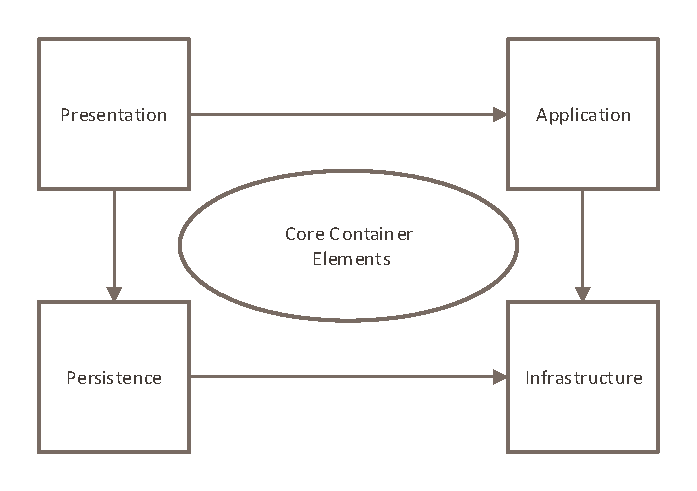
\includegraphics[width=\textwidth]{CoreElements}
\caption{Architecture Core Container Elements}
\label{fig:elements}
\end{figure}


\section{Architectural Drivers}
An analysis of the architectural drivers for each element was made following the techniques outlined by Wood \cite{Wood2007}. This analysis can be seen in appendix \ref{table:archdrivers}. Each requirements is analysed in accordance to its importance and impact or difficulty of implementation. This creates a combination of priorities as outlined by the case study and qualitative interpretation of research conducted. These priorities are then used to select the highest importance, highest impact drivers to architect first. 



